% Time-stamp: <09/10/02 01:57:13 vilhuber>
% $Id: Presentation-PSD.tex 3219 2012-09-27 07:47:11Z vilhu001 $

% normal line:
\documentclass[xcolor=table,compress]{beamer}
% to create notes:
%\documentclass[handout,notes=only]{beamer}
% to create handouts
%\documentclass[xcolor=table,handout,compress]{beamer}
% to create a different kind of handouts
%\documentclass{article}
%\usepackage[envcountsect]{beamerarticle}

%\setbeameroption{handout}
%\setbeameroption{show notes}


%
% Packages
%
\mode<article> % only for the article version
{
  \usepackage{fullpage}
  \usepackage{hyperref}
}
\usepackage{ifpdf}
\ifpdf
\usepackage{embedfile}
\embedfile{\jobname.tex}
\fi

\usepackage{graphicx}
%\usepackage{pstricks}
\usepackage{xcolor}
\usepackage{pifont}
%\usepackage{../chicago}
\usepackage{pgf}
\usepackage{amsmath,amssymb,amsfonts}
\usepackage[latin1]{inputenc}
\usepackage{colortbl}
\usepackage[english]{babel}
\usepackage{array}
\usepackage{pdfpages}
% usage:
%   \includepdf[pages={1}]{myfile.pdf}
%   \includepdf[pages={1,3,5}]{myfile.pdf} would include pages 1, 3, and 5 of the file. 
%   To include the entire file, you specify pages={-}, where {-}
%\usepackage{landscape}
\usepackage{listings}
\lstloadlanguages{R,bash,SAS}

%\usepackage{lmodern}
%\usepackage[T1]{fontenc}

\usepackage{times}
%\usepackage{colortbl}

%============================================================
% Beamer specific styles and configs
%============================================================

\mode<presentation>
{
% alternative, could always use
%\usetheme{Census}
\usetheme{cornell}
\useoutertheme{cornell}
}


%\setbeamercovered{dynamic}



%============================================================
% Title
%============================================================

\title[Computing for Economists]{Workshop: High-performance computing for economists}
\author[Vilhuber, Abowd, Mansfield, McKinney]{%
  Lars~Vilhuber\inst{1} \and
  John M. Abowd\inst{1} \and
  Richard~Mansfield\inst{1} \and
  Kevin~L.~McKinney %\inst{2}%
}

\institute[Cornell]{
  \inst{1}%
   Cornell University, Economics Department,
%\and \inst{2} U.S. Census Bureau
}%
\date[August 20-22, 2013]{August 20-22, 2013: Day 1}
\subject{HPC}


% % % % % % % % % % % % % % % % % Main document
\begin{document}
\frame{\titlepage}


\section[Intro]{Introduction}


\begin{frame}
Workshop: High-performance computing for economists
\end{frame}


\begin{frame}{HPC}
\begin{block}{Back in the days...}
\begin{center}
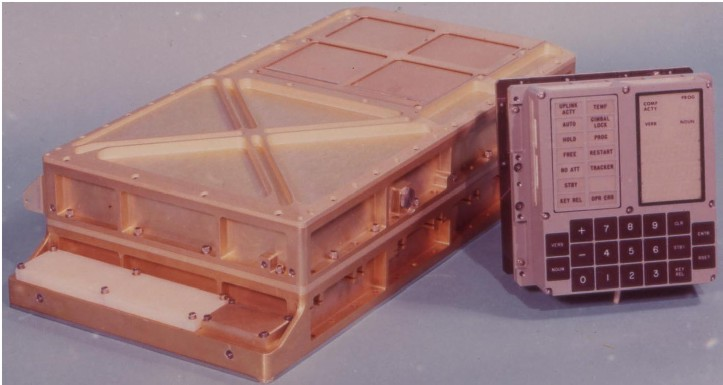
\includegraphics[height=0.6\textheight]{./Agc_view}
\end{center}
\end{block}
\pause
RAM: 2,000 words (2kB); Speed: 2 MHz
\newline
\tiny Source: \href{http://upload.wikimedia.org/wikipedia/commons/7/79/Agc_view.jpg}{Wikipedia}
\end{frame}

\begin{frame}{They went to the moon}
\begin{center}
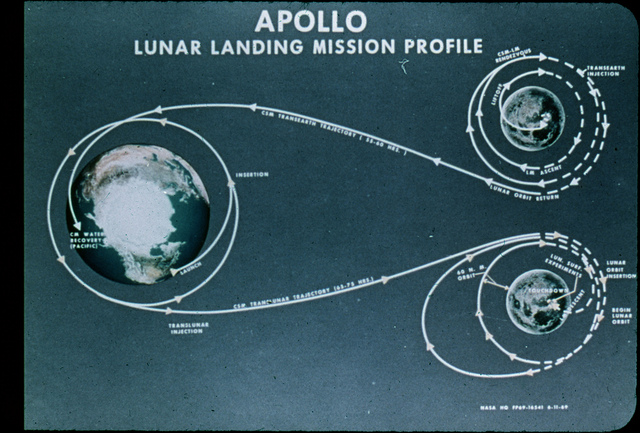
\includegraphics[height=0.7\textheight]{./apollo-11-path}
\end{center}
\tiny Source:  \href{http://farm2.staticflickr.com/1208/5105040212_346b792ee5_z.jpg}{Flickr}
\end{frame}


\begin{frame}{Big progress}
\begin{center}
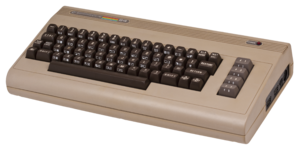
\includegraphics[height=0.7\textheight]{./300px-Commodore-64-Computer}
\end{center}
RAM: 2 $\times 32$ kB; Speed: 1 MHz, \$1,500 (today's USD)
\newline
\href{http://upload.wikimedia.org/wikipedia/commons/thumb/3/34/Commodore-64-Computer.png/300px-Commodore-64-Computer.png}{Wikipedia}
\end{frame}


\begin{frame}{Today}
\begin{center}
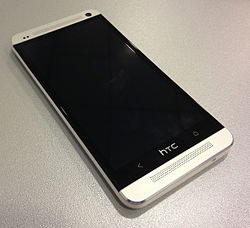
\includegraphics[height=0.7\textheight]{./HTC_One_Diagonal_View}
\end{center}
RAM: 2 $ \times 1024 ^2$ kB; Speed: 1.700 MHz $\times$ 4
\newline \$700 (today's USD) \tiny Source: \href{http://upload.wikimedia.org/wikipedia/commons/thumb/3/3d/HTC_One_Diagonal_View.jpg/250px-HTC_One_Diagonal_View.jpg}{Wikipedia}
\end{frame}


\begin{frame}{We still fly to the moon}
\begin{center}
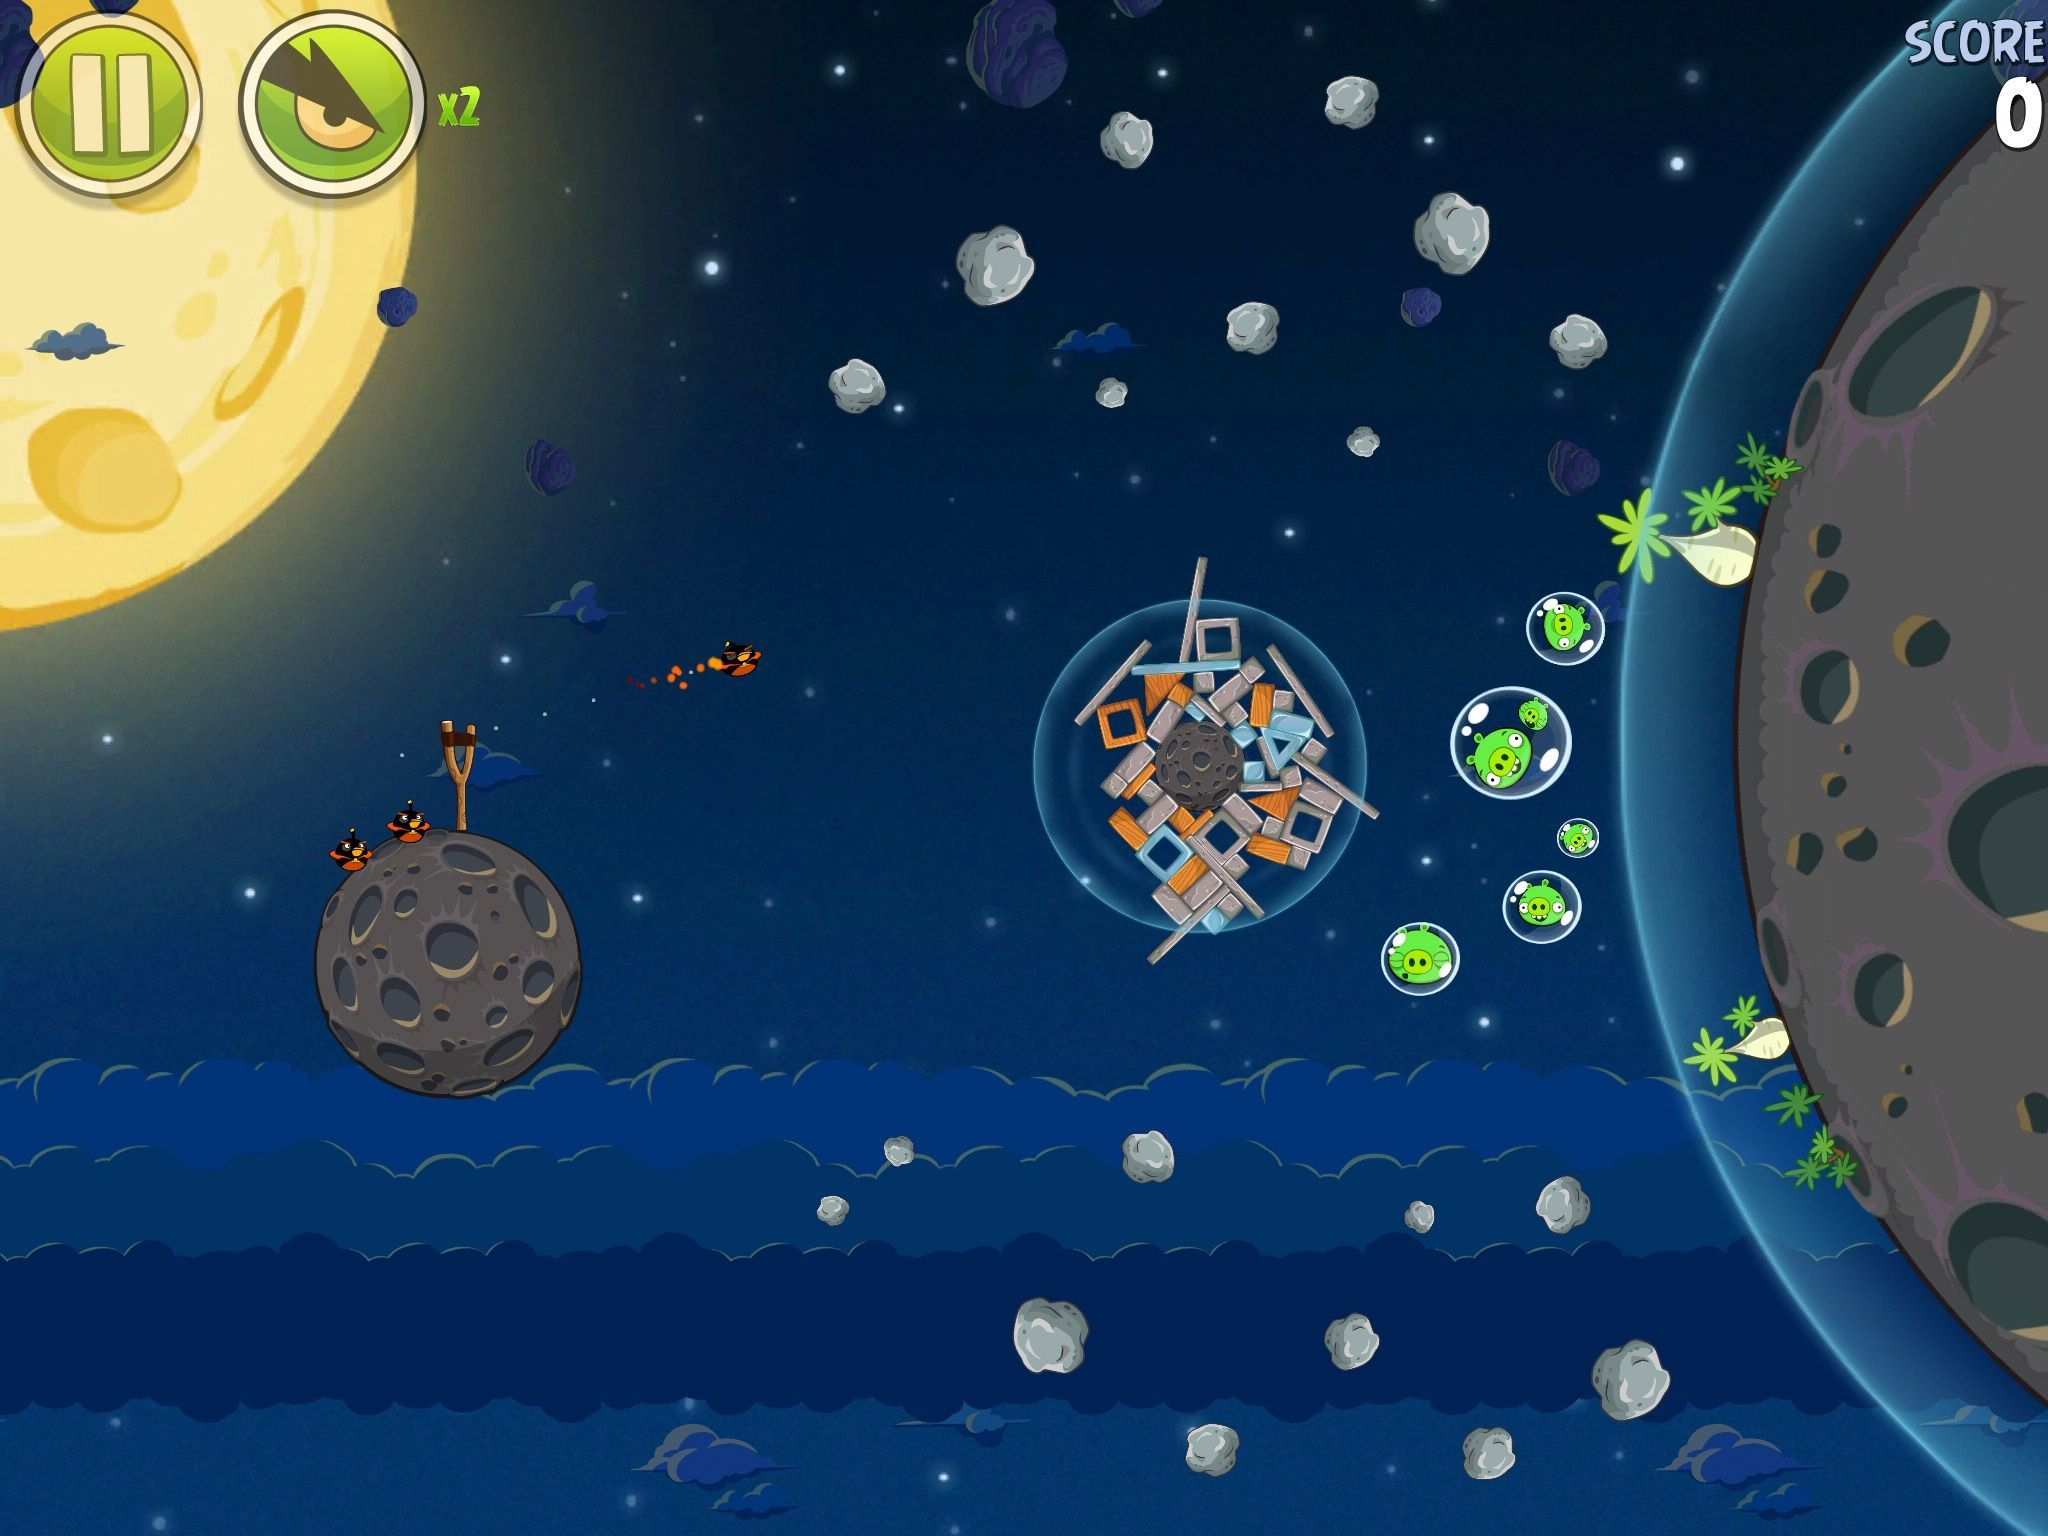
\includegraphics[height=0.7\textheight]{./Angry_Birds_Space_HD}
\end{center}
\tiny Source \href{http://i.i.cbsi.com/cnwk.1d/i/tim/2012/03/22/Angry_Birds_Space_HD.jpg}{CNET}
\end{frame}

\begin{frame}{This is where you can go}
\begin{block}{Stampede (no. 6 on Top500 as of June 2013)}
\begin{center}
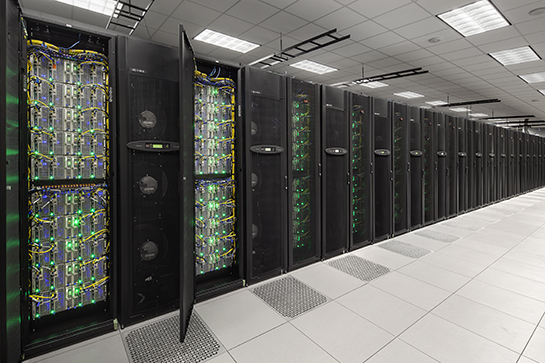
\includegraphics[height=0.5\textheight]{./stampede}
\end{center}\pause
RAM: 192 $\times 1024^3$ kB, Speed: 2,700 Mhz $\times$ {\Large 462,462}\newline
\tiny Source: \href{http://www.tacc.utexas.edu/image/image_gallery?img_id=714317&t=1362676291566}{TACC}
\end{block}
\end{frame}



\begin{frame}{But first...}
\pause
\begin{center}
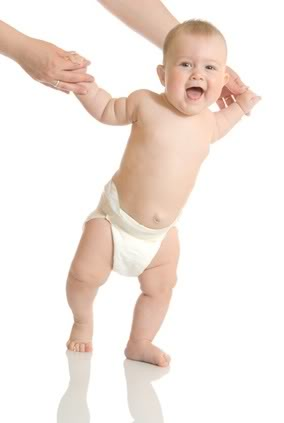
\includegraphics[height=0.8\textheight]{./baby-steps-one}
\end{center}
\tiny \href{http://viewfromwitsend.wordpress.com/}{http://viewfromwitsend.wordpress.com/}
\end{frame}


\begin{frame}
\begin{block}{What do you learn in a Ph.D. program?}
\pause
 How to learn...
\end{block}
\end{frame}

\begin{frame}
\begin{block}{Goal of this class}
\pause
To open new doors, to be able to conceive of problems that you didn't think had a feasible solution.\newline
\pause
To broaden your knowledge about what you do NOT know
\end{block}
\end{frame}

\subsection{Overview}
\begin{frame}{Overview}
\begin{block}{Day 1}
\begin{itemize}[<+->]
\item Programming basics (Lars)
\begin{itemize}
\item Choosing an editor
\item How to structure programs, texts, etc.
\item A clean sequence of programs
\item NX, SSH, Linux, request an account on cluster
\item Basic scripting
\end{itemize}
\item  Basics of version control (Lars)
\begin{itemize}
\item File-system based version control
\item More formal version control (Subversion, Git)
\item Working with servers
\item Setting up infrastructure at Cornell
\end{itemize}
\item Subroutines: the example of function programming in R (Lars)
\end{itemize}
\end{block}
\end{frame}

\begin{frame}{Overview}
\begin{block}{Day 2}

\end{block}
\end{frame}

\begin{frame}{Overview}
\begin{block}{Day 3}

\end{block}
\end{frame}

\subsection{Structure}

\begin{frame}{Structure of the class}
\begin{block}{Teaching...}
We'll take you on a 4,000 m flight through topics...
\end{block}
\pause
\begin{block}{... and practice}
... and then swoop in on some examples, leaving ample time to practice it.
\end{block}
\end{frame}

% % % % % % % % % % % % % % % End overview
\section[Basics]{Programming basics}
\subsection[Editors]{Choosing editors}

\begin{frame}{Choosing editors}
\begin{block}{Why does choosing editors matter?}
The (applied) research process iterates through writing papers and doing estimation. You want to use the appropriate tools for each task.
\end{block}
\begin{block}{Integrated or separate}
\begin{itemize}
\item You can use native tools that come with each word processing facility/programming language/etc. 
\item Not all of them will have one. 
\item Not all of them will work on all platforms.
\item You will likely use multiple tools
\end{itemize}
\end{block}
\end{frame}

\begin{frame}{Choosing an editor}
\begin{block}{... or system}
\begin{columns}[t]
\begin{column}{.48\textwidth}
\color{red}
Separate editors and systems 
\begin{itemize}
\item MS Word and math editor (Windows/OSX but compatibility issues)
\item \href{http://www.libreoffice.org}{LibreOffice} (Windows/OSX/Linux but not as good)
\item NotePad++ (Windows)
\item Gedit, (X)Emacs, Kate (Linux)
\item ?? (OSX)
\end{itemize}
\end{column}
\hfill
\begin{column}{.48\textwidth}
{\color{red}
\LaTeX}: all platforms, but some GUIs are not cross-platform, ease of use varies:
\begin{itemize}
\item TeXstudio (all platforms)
\item TeXMaker (all platforms)
\item Scientific Workplace (Windows, mythical Linux) 
\item \href{http://www.tug.org/texworks/}{TeXWorks}+\href{http://miktex.org/}{Miktex}
\item \href{http://www.texniccenter.org/}{TEXnicCenter}
\item and  (\href{http://alternativeto.net/software/texmaker/}{many more})
\end{itemize}
\end{column}
\end{columns}
\end{block}
\end{frame}



\begin{frame}{Choosing an editor}
\begin{block}{... or system}
\begin{columns}[t]
\begin{column}{.48\textwidth}
\color{blue}
Integrating programming and running
\begin{itemize}
\item \href{http://en.wikipedia.org/wiki/Integrated_development_environment}{IDE} ( \href{http://en.wikipedia.org/wiki/Eclipse_(software)}{Eclipse}, \href{http://en.wikipedia.org/wiki/ActiveState_Komodo}{ActiveState Komodo}, etc.)
\item Native programming GUIs (SAS, Matlab, Stata)
\item Gedit, (X)Emacs (with add-on functionality)
\end{itemize}
\end{column}
\hfill
\begin{column}{.48\textwidth}
\color{blue}
Integrating programs and text/results
\begin{itemize}
\item SWeave (integrates \LaTeX \ and R)
\item RStudio (GUI to R and SWeave)
\item StatRep (Integrated SAS and \LaTeX, \href{http://support.sas.com/resources/papers/proceedings12/324-2012.pdf}{Source 1}, \href{http://support.sas.com/StatRepPackage}{Source 2})
\end{itemize}
\end{column}
\end{columns}
\end{block}
\end{frame}

%=======================================================================
\subsection[Structure]{Structuring programs and texts}

\begin{frame}[fragile]{Structuring programs}
\begin{block}{Easy...}
\lstset{numbers=left, stepnumber=1,  language=SAS, basicstyle=\tiny,
caption=mystuff.sas}
\begin{lstlisting}
data "C:\Users\Me\CensusChina.sas7bdat";
     set "C:\Users\Me\CensusChina.sas7bdat";
     earn=log(earn);
run;
proc reg data="C:\Users\Me\CensusChina.sas7bdat";
model earn = sex education experience;
run;
\end{lstlisting}
What can possibly be wrong about that?
\end{block}
\end{frame}

\begin{frame}[fragile]{Structuring programs 2}
\begin{block}{Easier...}
\lstset{numbers=left, stepnumber=1,  language=SAS, basicstyle=\tiny,
caption=mystuff.do}
\begin{lstlisting}
use "C:\Users\Me\CensusChina.dta"
replace  earn=log(earn)
regress  earn  sex education experience
save, replace
\end{lstlisting}
What can possibly be wrong about that?
\end{block}
\end{frame}



\begin{frame}{Structuring programs 3}
\begin{block}{Actually...}
{\Large Everything!}
\begin{itemize}
\item Name of program: uninformative
\item Destruction of original data: program cannot be re-run for same results
\item No portability: cannot be run anywhere else
\item No explanation: why are we doing this?
\end{itemize}
\end{block}
But of course, nobody does that, right?
\end{frame}


\begin{frame}[fragile]{Structuring programs 4}
\begin{block}{Better...?}

\lstset{numbers=left, stepnumber=1,  language=SAS, basicstyle=\tiny,
caption=china-regression.sas}
\begin{lstlisting}
data logCensusChina;
     set "C:\Users\Me\CensusChina.sas7bdat";
     earn=log(earn);
run;
proc reg data=logCensusChina;
model earn = sex education experience;
run;
\end{lstlisting}
\pause
Somewhat...
\end{block}
\end{frame}




\begin{frame}{Structuring programs 5}
\begin{block}{Addressing these issues}
\begin{itemize}
\item Naming of programs: here
\item Commenting: here
\item Versioning: \href{day1-2.pdf}{up next}
\item Portability and Data management: tomorrow
\end{itemize}
\end{block}
\end{frame}



\begin{frame}{Key notions about naming}
\begin{block}{Think of yourself as highly amnesiac...}
\begin{itemize}[<+->]
\item The research paper you are writing now will be submitted, rejected, worked on, questioned... 
\item ... by others and yourself
\item ... in intervals of weeks, months, years...
\item Your future research assistant and the future YOU will need to understand how to go through it.
\end{itemize}
\end{block}
\end{frame}



\begin{frame}[fragile]{Naming}
\begin{block}{The really bad}
\begin{lstlisting}[language=bash,numbers=none]
mystuff.R
read.R
version2.R
ols.sas
\end{lstlisting}
\end{block}
\pause
\begin{block}{The bad}
\begin{lstlisting}[language=bash,numbers=none]
readCensus.R
readBLS.R
prepareCensus.R
runOLS.sas
\end{lstlisting}
\end{block}
\end{frame}



\begin{frame}[fragile]{Naming}
\begin{block}{Better}
\begin{lstlisting}[language=bash,numbers=none]
01_readBLS.R
02_readCensus.R
03_prepareCensus.R
04_create_analysis_data.R
05_runOLS.sas
\end{lstlisting}
\end{block}
\pause
\begin{block}{Even better}
\begin{lstlisting}[language=bash,numbers=none]
01_01_readBLS.R
02_01_readCensus.R
02_02_prepareCensus.R
03_01_create_analysis_data.R
04_01_runOLS.sas
README.txt
\end{lstlisting}
\end{block}
\end{frame}


\begin{frame}[fragile]{Naming}
\begin{block}{Going overboard?}
\begin{lstlisting}[language=bash,numbers=none,basicstyle=\tiny]
icf/ctrlprogs/control_icf.sas
icf/ctrlprogs/parameters_icf.sas
icf/library/macros/icf_cleanup.sas
icf/library/macros/icf_impute_county_res.sas
icf/library/macros/licf_findnum.sas
icf/library/macros/licf_proxy.sas
icf/library/macros/licf_stars1.sas
icf/library/macros/licf_tgrlatlongs.sas
icf/library/sasprogs/01_icfqa.sas
icf/library/sasprogs/01_icf.sas
icf/library/sasprogs/02_icfqa.sas
icf/library/sasprogs/02_icf.sas
icf/library/sasprogs/03_icfqa.sas
icf/library/sasprogs/03_icf.sas
[snip]
icf/library/sasprogs/19_icf.sas
\end{lstlisting}
\pause
\begin{lstlisting}[language=bash,numbers=none,basicstyle=\tiny]
ehf/ctrlprogs/control_ehf.sas
ehf/library/macros/read_bls.sas
ehf/library/sasprogs/01_ehf.sas
[snip]
\end{lstlisting}
\end{block}
\end{frame}


\begin{frame}[fragile]{Naming}
\begin{block}{With minor modification}
\begin{lstlisting}[language=bash,numbers=none,basicstyle=\tiny]
icf/ctrlprogs/control_icf.sas
icf/ctrlprogs/parameters_icf.sas
icf/library/macros/icf_cleanup.sas
icf/library/macros/icf_impute_county_res.sas
icf/library/macros/licf_findnum.sas
icf/library/macros/licf_proxy.sas
icf/library/macros/licf_stars1.sas
icf/library/macros/licf_tgrlatlongs.sas
icf/library/sasprogs/01_icf.sas
icf/library/sasprogs/02_icf.sas
icf/library/sasprogs/03_icf.sas
[snip]
icf/library/sasprogs/19_icf.sas
icf/library/sasprogs/01_icfqa.sas
icf/library/sasprogs/02_icfqa.sas
icf/library/sasprogs/03_icfqa.sas
\end{lstlisting}
Can you figure out in what sequence to run them?
\end{block}
\end{frame}



\subsection{Getting access to a compute cluster}

\begin{frame}
\begin{block}{Linux}
\begin{itemize}
\item used on most compute clusters
\item used on very few desktop computers
\item but...
\end{itemize}
\end{block}
\pause
\begin{block}{Bash}
\begin{itemize}
\item bash is a ``shell'' - a text interface command interpreter
\item bash or ksh (Korn shell) or csh (C-shell) are the most common
\item bash is available on Linux and \pause OSX
\item you can also download Cygwin, getting bash for Windows
\end{itemize}
\end{block}
\end{frame}

\begin{frame}{Access to your local compute cluster}
\begin{block}{Several on-campus compute resources}
\begin{itemize}[<+->]
\item Cornell Center for Advanced Computing (\href{http://www.cac.cornell.edu}{CAC})\newline \uncover<3->{\alert{$\rightarrow$ Thursday}}
\item Cornell Institute for Social and Economic Research (\href{http://www.ciser.cornell.edu}{CISER})\uncover<3->{\alert{$\rightarrow$ Thursday}}
\pause
\item Economics Compute Cluster Organization (ECCO), aka Social Science Gateway (SSG)
\end{itemize}
\end{block}
\end{frame}


\begin{frame}{Getting access to ECCO}
\begin{block}{You already have...}
\begin{itemize}
\item You have an account by virtue of participating in this class
\item Moving forward, you will be eligible to faculty-sponsored accounts
\item Currently soft-monitoring of resource usage
\end{itemize}
\end{block}
\pause
\begin{block}{... but do you have \textbf{access}?}
Have you logged in via SSH to reset your password? \newline \uncover<3->{\alert{$\rightarrow$ \href{http://www2.vrdc.cornell.edu/news/ecco/step-2-first-login/}{Instructions}}}
\end{block}
\end{frame}


\begin{frame}{Quick walkthrough, using Chrome SSH}
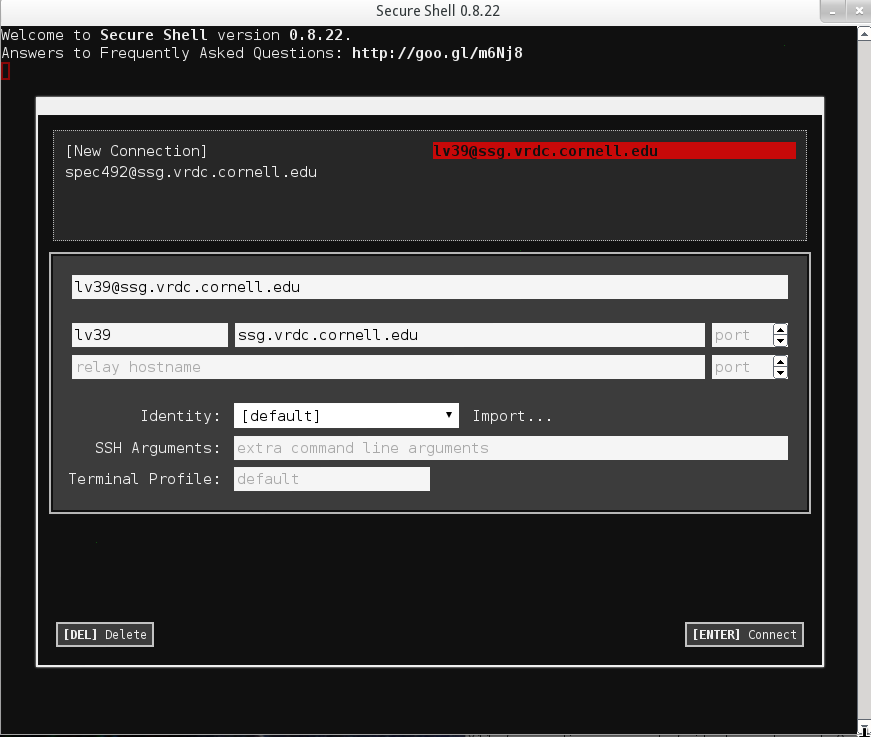
\includegraphics[width=.9\textwidth]{chrome-ssh-screen1.png}
\end{frame}


\begin{frame}{Quick walkthrough, using Chrome SSH}
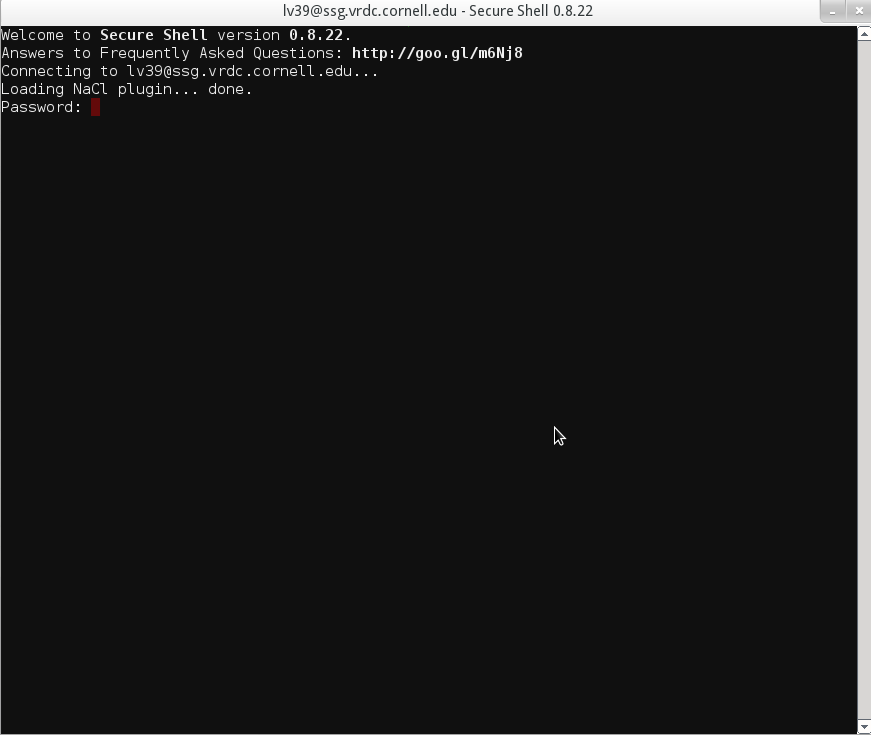
\includegraphics[width=.9\textwidth]{chrome-ssh-screen2.png}
\end{frame}


\begin{frame}{Quick walkthrough, using Chrome SSH}
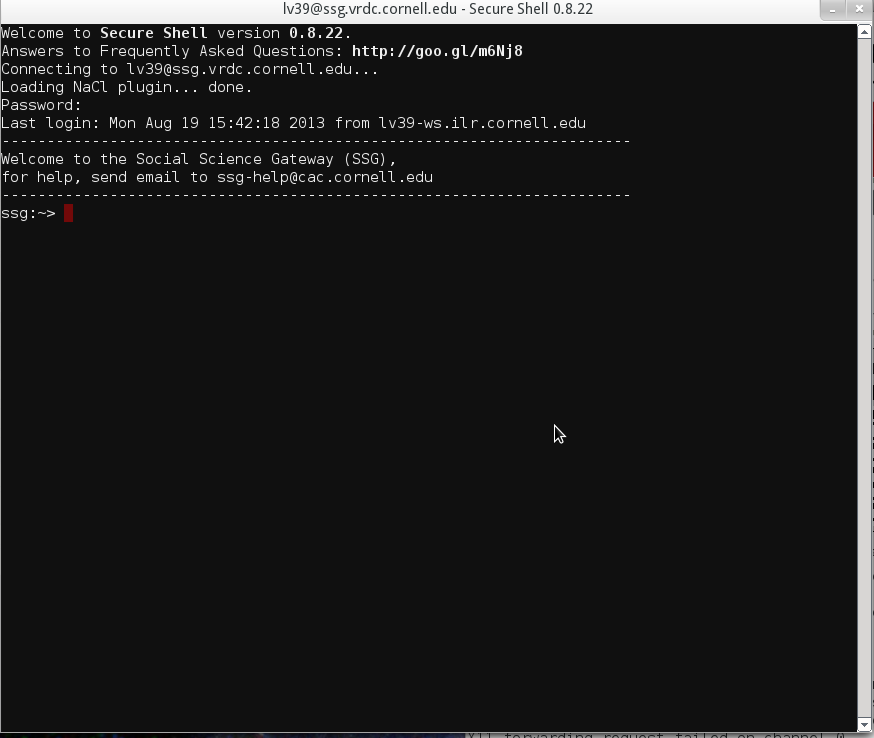
\includegraphics[width=.9\textwidth]{chrome-ssh-screen3.png}
\end{frame}


\begin{frame}{Why SSH?}
\begin{block}{Most compute clusters have ONLY SSH access}
It is thus worthwhile to learn enough about it here, in order to be functional there: CAC ``Red Cloud'', Amazon Cloud, XSEDE. 
\end{block}
\begin{block}{Linux rules... the HPC world}
All 10 of the top 10 \href{http://www.top500.org/list/2013/06/}{TOP500} computers run Linux (as the compiler front-end, if not compute OS)
\end{block}
\end{frame}



\begin{frame}{Graphical access}
\begin{block}{Two types of graphical access}
\begin{itemize}[<+->]
\item with an ``X server'' (native in Linux, optional in Windows and OSX) \uncover<2->{\alert{$\rightarrow$ standard way on most clusters}}
\item<3-> using NX client software for improved experience
\end{itemize}
\end{block}
\end{frame}



\begin{frame}{Access via NX}
\begin{block}{What is NX?}
NX is software similar to Windows Remote Desktop, allowing for a graphical interface to be made available remotely.
\end{block}
\begin{itemize}
\item Client is free (provided by Nomachine)
\item We use a free server (not provided by Nomachine, but fully functional)
\item Clients can be launched by installing dedicated client (all OS)  or by launching the webclient (currently not working for some Linux)
\end{itemize}
\end{frame}


\begin{frame}{Important note}
\begin{block}{NX on ECCO security}
You MUST download the custom-configured session from the VRDC website; the default session configuration from the NX client install will not work.
\end{block}
\tiny Details: we use a custom SSH key for the NX client, for some minimal additional security.
\end{frame}


\begin{frame}{Important note}
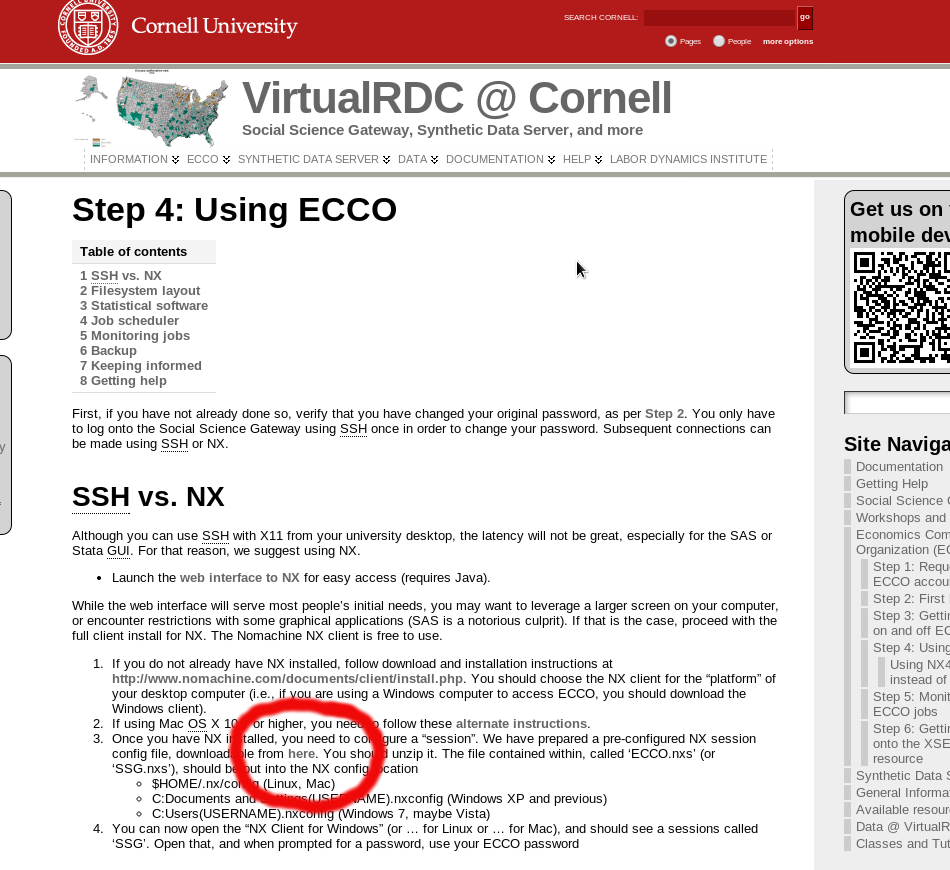
\includegraphics[height=.7\textheight]{nx-ecco-key.png}
\end{frame}


\begin{frame}{Logging on}
\centering
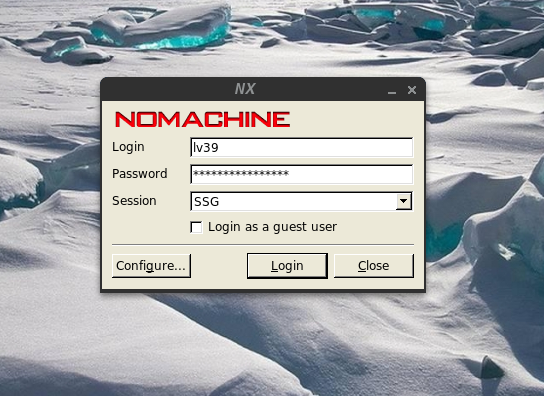
\includegraphics[height=.7\textheight]{nx-login-box.png}
\end{frame}


\begin{frame}{Successful connection}
\centering
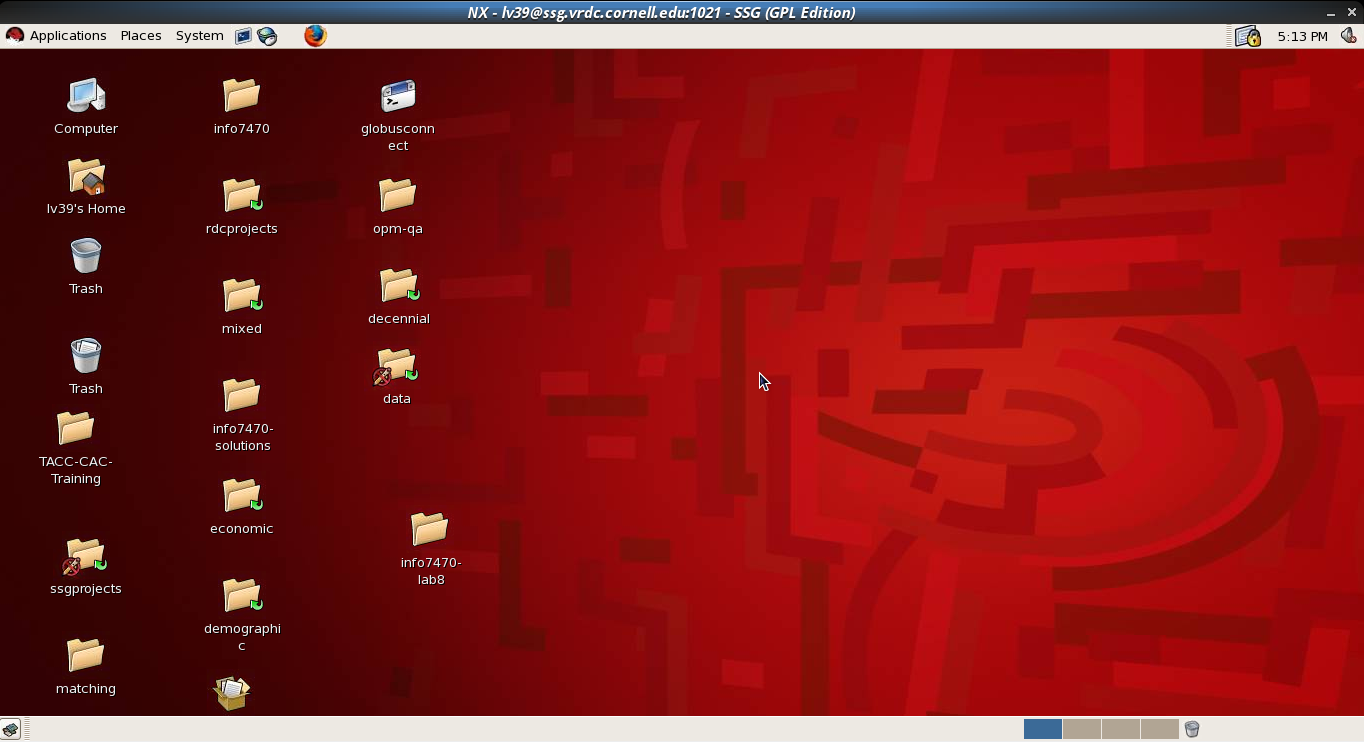
\includegraphics[width=1\textheight]{nx-logged-on.png}
\end{frame}


\subsection{Basic scripting}

\begin{frame}
Basic Linux, basic scripting
\end{frame}


\begin{frame}{Why worry?}
\begin{block}{You will end up doing something on the command line}
\begin{itemize}[<+->]
\item Launch a program from a compute-cluster job
\item Launch a job submission
\item Basic scripting
\end{itemize}
\end{block}
\end{frame}

\begin{frame}[frame]{Linux in 2 minutes}
\begin{itemize}
\item ls - will list the contents of a directory
\item cd - will ``change directory''
\item cd .. (note the spaces) will go up a directory
\item cd (name) will go into the directory (name)
\item rm (name) will delete
\item mkdir (name) will create a directory called (name)
\item vi (name) will open a venerable command line editor for file (name) \pause (CAUTION: to exit, hit ESC, then :q!)
\end{itemize}
\end{frame}


\begin{frame}[fragile]{Basic scripting in Linux}
\begin{block}{A basic loop on the command line}
\lstset{numbers=left, stepnumber=1, frame=single, language=bash}
\lstinputlisting{../programs/day1/1-1-basic-loop.bash}
\end{block}
\tiny{Source: \href{http://www.cyberciti.biz/faq/bash-for-loop/}{[1]}}
\end{frame}

\begin{frame}[fragile]{Capturing output}
\begin{block}{You can capture the output from a command}
\begin{lstlisting}
> seq 1 3
1
2
3
\end{lstlisting}
Now let's use that:
\begin{lstlisting}
for i in $(seq 1 3)
do
  echo $i
done
\end{lstlisting}
\end{block}
\end{frame}


\begin{frame}[fragile]{Basic scripting in Linux}
\begin{block}{Use for practical things}
Remember that ICF program sequence? How would we go about starting 19 programs in sequence?
\begin{lstlisting}
for program in $(ls *_icf.sas)
do
  sas $program
done
\end{lstlisting}
\end{block}
\end{frame}


\begin{frame}{Advanced linux in 2 minutes}
\begin{block}{The gateway to everything}
{man}
\end{block}
or try \href{http://www.linuxmanpages.com}{http://www.linuxmanpages.com} or \href{http://linux.die.net/man/}{http://linux.die.net/man/}
\begin{block}{The toolkit}
\begin{itemize}
\item sed
\item grep
\item awk
\item regex (regular expressions)
\end{itemize}
\end{block}
\end{frame}


\begin{frame}[fragile]{Advanced scripting in Linux}
\begin{block}{Use for practical things}
What if I'm running 100s of programs, and trying to figure out
if any of them have errors?
\begin{lstlisting}
for logfiles in $(ls *_icf.log)
do
  grep ERROR $logfiles
done
\end{lstlisting}
\end{block}
\end{frame}





\begin{frame}
Now let's try it out
\end{frame}

\section[VCS]{Version control systems}
\begin{frame}
\href{day1-2.pdf}{Next section}
\end{frame}

\section{Subroutines}
\begin{frame}
\href{day1-3.pdf}{Next section}
\end{frame}

\end{document}